\section{Introduction}

This study is a partial replication of Geerts, Chersi, Stachenfeld and Burgess (2020) \cite{Geerts:2020} that presented a reliability-based arbitration mechanism between an associative-learning strategy and a place-based navigation strategy. This model was proposed to mimic the behavior of rats in a series of spatial navigation tasks that had been reported in previous experimental articles.

The associative-learning strategy is implemented using a classical Q-learning algorithm which is fed with visual input in an egocentric frame of reference. The place-based strategy on the other hand works in an allocentric fashion and is implemented using the Successor-Representation initially proposed by Peter Dayan (1993) \cite{Dayan:1993}.

Here we present replications of model simulations in the first task addressed by Geerts and colleagues \cite{Geerts:2020}, i.e, the Pearce, Roberts and Good (1998) experiment \cite{Pearce:1998}. This task is a variant of the Morris water-maze task \cite{Morris:1982}. In this experiment, the behavior of a group of hippocampally-lesioned animals is compared with that of a control group while they have to find a hidden platform immerged under opaque water. The platform location is indicated by a nearby visual landmark, while the position of the platform is regularly moved across multiple trials and sessions, to force the animals to constantly adapt (Fig.~\ref{fig:maze}.A).

Geerts and colleagues provided a python implementation of their model and of the simulated task, accessible on ModelDB \cite{modeldb}. Nevertheless, we were not able to reproduce their results without modifications to the original code and model parameters. Furthermore, while inspecting the provided modules, we found several discrepancies with the original experimental protocol (Fig.~\ref{fig:maze}.B).


In summary, although we partly reuse the original code of Geerts et al. (2020) \cite{Geerts:2020}, we argue that the present work should be considered as a replication rather than as a reproduction (see \href{https://rescience.github.io/faq/}{the ReScience FAQ} for a discussion on the meaning of both of these terms) due to the numerous changes brought to both the navigation strategy models and to the simulated experimental protocol.

\begin{figure}[htp]
    \centering
    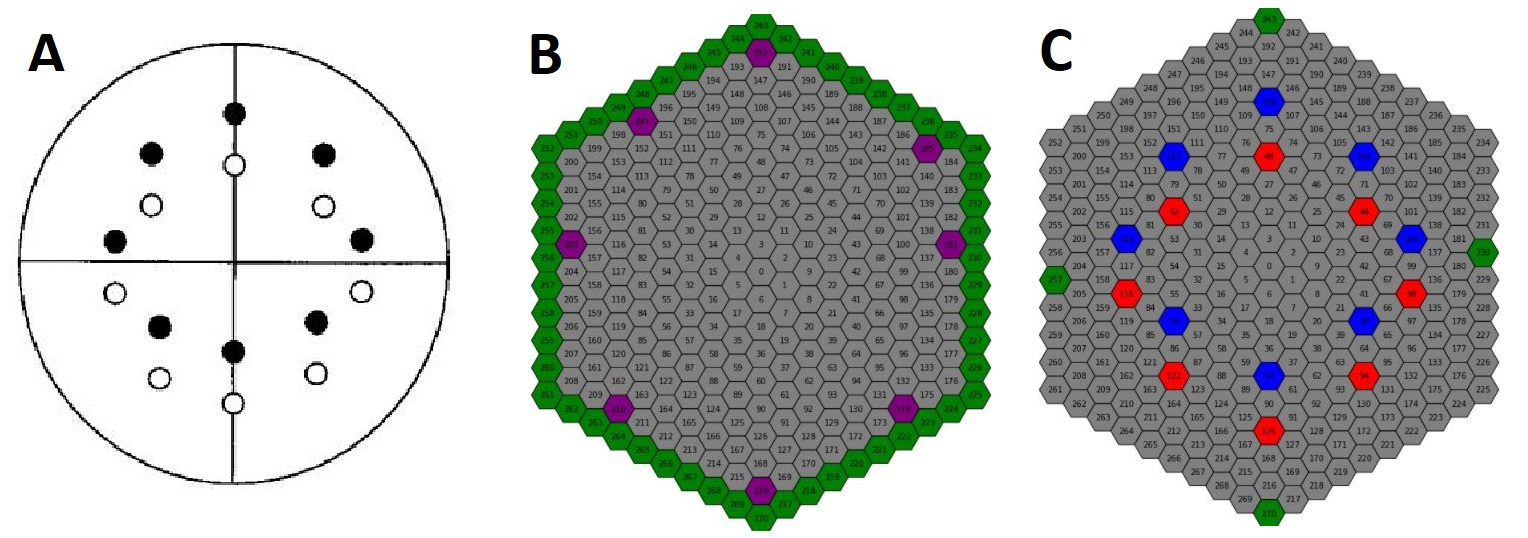
\includegraphics[width=12cm]{Geerts_Original_Maze2.JPG}
    \caption{{\bf A}: Original design of the water maze. Possible positions of the platforms represented as white circles, while their associated landmarks are represented as black circles. From Pearce et al., (1998) {\bf B}: Geerts et al. (2020)'s version of the maze. Platforms and landmarks represented in purple on the same states, though there is actually half a state (5cm) that separate them. Eligible starting states in green. {\bf C}: Our version of the maze. Platforms in red, landmarks in blue, starting states in green.}
    \label{fig:maze}
\end{figure} 

\section{Methods}

\subsection{Pearce, Roberts and Good (1998) experimental protocol}
In this experiment, rats were released in a circular tank (pool) filled with opaque water (Fig.~\ref{fig:maze}.A). They had 120 seconds to swim and find an immersed platform on which they could rest for 30 seconds, before being subjected to a new trial of the experiment. Animals that did not find the platform after 120 seconds were lifted from the water by the experimenter and placed back on the platform for 30 seconds.

A spherical black landmark was placed, distant from a fixed offset of 20 centimeters to the north of the platform. This helped the animal roughly localize the area were the platform was located, while not enabling rats to simply use a cue-guided strategy because of the distance between the landmark and the platform. This was meant as a means to make rats use a combination of a cue-guided (associative learning) strategy and a place-based strategy relying on hippocampus-based mapping of the environment thanks to the distal landmarks placed around the pool. The pool, platform and landmark were respectively of a 2m, 10cm and 13cm diameter.

Two groups of rats were tested: a control group and a hippocampal-lesioned group. Each animal was subjected to eleven sessions of four trials each. At each new session, the platform and the landmark were moved to a new location inside the maze, both always conserving their relative positioning (Fig.~\ref{fig:maze}.A).

In their original article, Pearce, Roberts and Good \cite{Pearce:1998} measured at each trial the total time it took for the rats to find and climb on the hidden platform from the moment they were released in the water at one of the four possible starting points (illustrated in Fig.~\ref{fig:maze}.C).  The authors results can be summarized into three main behavioral properties illustrated by the learning curves: (1) Only control rats were able to significantly learn within a session of four trials, thus indicating that an intact hippocampus is required to adapt to a change in goal location within such a short amount of time. (2) At the first trial of each session, the escape time was smaller for the hippocampal-lesioned group than for the control group; further analyses (not shown here) suggested that an intact hippocampus makes animals lose time at the previous platform location, which was later confirmed by previous computational modeling work applied to this task \cite{Dolle:2018}. (3) The learning curves of both groups at both Trial 1 and Trial 4 progressively converged to the same escape latency at Session 11 (Fig.~\ref{fig:learningCurves}.A).


\begin{figure}[htp]
    \centering
    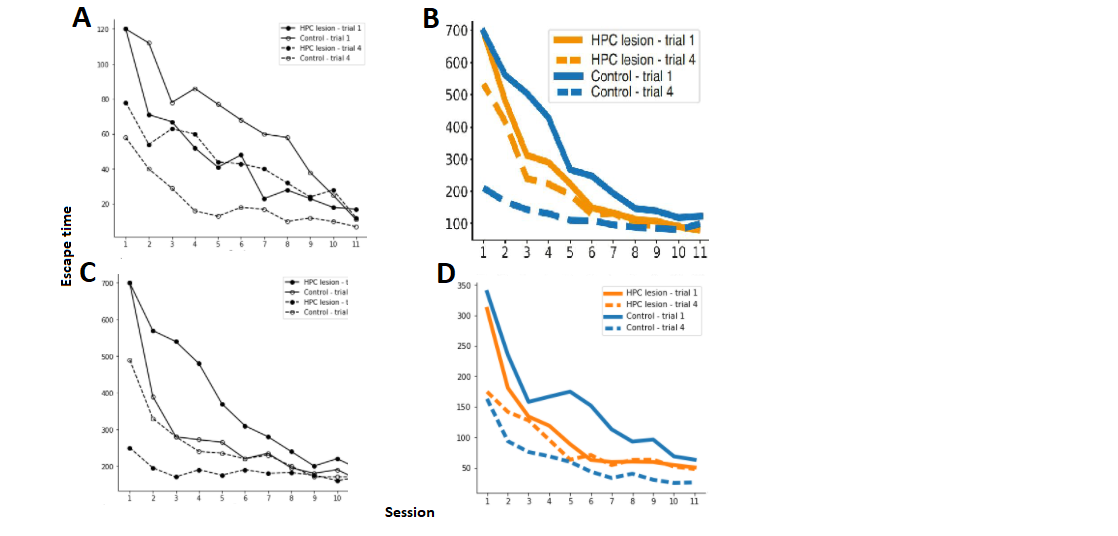
\includegraphics[width=20cm]{results.png}
    \caption{Mean escape-time across sessions. 
    {\bf A} Experimental results from Pearce. 
    {\bf B} Results published in Geert et al. (2020)'s article, continuous lines represent performances on the first trial of each session, doted lines represent the last trial. Blue lines indicate control group performances, whereas orange is linked with the hippocampally-lesioned group. 
    {\bf C} Our reproduction of Geerts et al. (2020)'s results after optimizing model parameters in their version of the simulated task illustrated in Fig.~\ref{fig:maze}.B. Processing time for 100 agents: 4h07min.
    {\bf D} Our replication of Geerts et al. (2020)'s results after optimizing model parameters in the adapted version of the simulated task illustrated in Fig.~\ref{fig:maze}.C.
    Processing time for 100 agents: 21 minutes.}
    \label{fig:learningCurves}
    
\end{figure}

\subsection{Topological discrepancies with Geerts, Chersi, Stachenfeld and Burgess (2020)'s provided code}
Geerts et al. (2020)'s computational version of the water-maze consists of an hexagonal environment composed of 271 discrete states (see Figure~\ref{fig:maze}.B). Transitions from one state to its neighbors are possible along six directions: North, North-East, South-East, South, South-West and North-West. 

A first topological discrepancy with the original experiment is that in the latter the landmark-platform distance is of a constant 20cm. In contrast, in Geerts et al. (2020)’s code this distance is only of half a state, which roughly represents 5 centimeters relative to the size of the maze. This is quite important as these 20 centimeters distance were originally introduced by Pearce et al. (1998) to prevent a simple cue-guided learning strategy to be sufficient to solve the task: such a strategy would not have been sufficient for the animal to find the platform by chance when moving around the landmark. A substantial distance between landmark and platform is thus important to hinder rats’ associative-learning performances, and thus to ensure that they would also rely on their cognitive mapping abilities. 

Secondly, in Geerts et al. (2020)’s version of the task, agents are released from any of the states that are adjacent to the border of the pool, as long as the distance from the release point of the previous trial is sufficiently large. In contrast, in the original protocol agents were released at each trial from a random combination of all the four cardinal states.

Finally, the platform's positions provided in Geerts et al. (2020)’s source code were not accurately enough replicating the original topology of the environment. Indeed, Pearce and colleagues indicated that in the original protocol « the landmark and the platform midpoint was always located at the middle of one of the eight radii that were oriented toward the eight main points of the compass » (Pearce et al., 1998) \cite{Pearce:1998}. In contrast, as can be seen on Figure~\ref{fig:maze}.B, Geerts and colleagues positioned the platform too close to the edge of the pool. As a result, agents have a higher probability of reaching the platform by chance when navigating along the pool border.

These three topological discrepancies have all been corrected in our new implementation. Our version of the maze can be visualized and compared to the others in Figure~\ref{fig:maze}.C.

\subsection{Non-topological discrepancies and limitations in the implementation of the navigation strategies}

In Geerts et al. (2020)’ code, the agents’ Successor-Representation module was instantiated with non-random and non-zero weights. The weights were instantiated in such a way that the SR encoded an optimal representation of the transition function, as if agents had already wandered around across the water-maze in an initial latent learning phase. Such a phase, however, is absent from the original protocol described in Pearce et al. (1998)'s article. We corrected this by setting the initial values of all elements of the SR's matrix to 0.

Secondly, Geerts et al. (2020)’s protocol did not implement a mechanism simulating a laboratory assistant picking up the rat and placing it on the platform after failure of the rat to find it on its own. We thus implemented a mechanism which allows an agent in this situation to actually experience a transition to the platform state.

Another important limitation of Geerts et al. (2020)'s simulated results, which prevents them from perfectly reproducing rats' behavior in Pearce et al. (1998) has to do with the performance asymptote of the learning curves (Fig.~\ref{fig:learningCurves}.B). More precisely, the curves in Figure~\ref{fig:learningCurves}.B converge to a mean espace time of about 100 iterations of the model (to be compared with the <50 model iterations we reached after parameter optimization; Fig.~\ref{fig:learningCurves}.D). This means that the final performance of the originally simulated agents was not optimal, and that they followed detouring paths towards the platform, in contrast to the rat behavior reported in Pearce et al. (1998).

In addition, a more minor discrepancy of Geerts et al. (2020)'s simulations has to deal with the agents' limited visual perception. Their source code contains two consecutive uncommented lines, one which limits agents' ability to perceive the intra-maze landmark at distances higher than 180 cm, and the next line which limits it further to 60 cm. First, it is not clear which of the two limits was used in the simulations presented in Geerts et al. (2020), since this parameter of their simulations is not discussed in the paper. Nevertheless, given that the two lines are uncommented, it is likely that the simulated rats' perception was restricted to less than 60-cm distances. While it is known that rats' visual acuity is poor compared to humans \citep{caves2018}, it is unlikely that in the original experiment rats were not able to perceive the visual landmark above 60-cm distances. This is important, as the agents' distance from the landmark can go up to 150 cm in Pearce et al. (1998)'s experiment. This 60-cm limit can thus make the associative-learning strategy perform artificially poorly. In contrast, from the detailed description of the experimental protocol of Pearce and colleagues \citep{roberts1998}, it is clear that the intramaze landmark is visually salient for the rats, since it is painted in black while the pool's walls are painted in white. Moreover, the experimental results show that rats can also take into account the extramaze visual cues (posters with salient colors on the wall of the 4mx3m experimental room, and a computer screen), while these distal cues are located at least 30 cm away from the pool's edge, and up to 1 m away. For these reasons, we increased the visual field of the landmark neurons in the associative-learning module to 260cm.

Finally, there was in the code no trace of an implementation of the eligibility trace algorithm, as claimed in the methods of the paper. We did not implement one in our version.

\subsection{Required re-optimization of model parameters}
In order to first reproduce Geerts et al. (2020)'s simulation results \citep{Geerts:2020} with the same virtual maze that they used (depicted in Fig.~\ref{fig:maze}.B), we executed the original script provided by the authors. We were able to execute the code after correcting a few minor bugs. 
On the other hand, the parameters presented in the article are different from those found in the original source code of Geerts and colleagues. Thus it was not clear which exact model parameters were used to produce Fig.~\ref{fig:learningCurves}.B (adapted from their article). We were unable to replicate the authors learning curves with either parameter-sets, thus we used manual tuning to find a suitable combination of parameter values.

Secondly, as we modified the simulated protocol to better match Pearce's task (Fig.~\ref{fig:maze}.C), we had to  perform a parameter optimization so as to try to fit and replicate the experimental data (Fig.~\ref{fig:learningCurves}.A) Specifically, we ran a random grid-search on four of the model's parameters: SR learning rate, MF learning rate, value function discount rate and exploration inverse temperature. We generated 2000 random combinations of these four parameters within bounded values. We then conducted a single agent simulation for each set of parameters. The mean performances of local clusters of datapoints in the four dimensional-space of parameters was computed and compared to the experimental data using the Mean-Squared-Error (MSE) method. The centroid of the cluster with the lowest MSE was selected to produce the data published in this paper (Fig.~\ref{fig:learningCurves}.D).

\section{Results}





We were first able to reproduce Geerts and colleagues' results using their original code (see Fig.~\ref{fig:learningCurves}.C). Nevertheless, this required a new optimization of model parameters (Table.~\ref{tab:param}), as neither those provided in the article nor in the code were able to match the article's figure (Fig.~\ref{fig:learningCurves}.B). 

\begin{center}
\hspace*{-1cm}
\begin{tabular}{ |c|c|c|c|c| }

\hline
Parameters & Geerts article & Geerts code & Reproduction & Replication \\ [0.5ex] 
\hline\hline
Maze size (diameter) & Unspecified  & 10 states & 10 states  & 10 states\\ 
Number of agents & Unspecified & 100 & 100 & 100\\ 
Platform-landmark distance & Unspecified & 1 state & 1 state & 4 states\\ 
HPC module learning rate & 0.07 & 0.1 & 0.07 & 0.074\\
DLS module learning rate & 0.07 & 0.1 & 0.07 & 0.256\\
Arbitrator inverse temperature & 5 & 5 & 16 & 50\\
SR Discount factor & 0.95 & 0.99 & 0.95 & 0.82 \\
DLS Discount factor & 0.95 & 0.9 & 0.9 & 0.92 \\
Reliability learning rate & 0.03 & 0.03 & 0.03 & 0.03 \\
Transition rate MF to SR & Unspecified & 0.01 & 0.01 & 0.01 \\
Transition rate SR to MF & Unspecified & 0.1 & 0.1 & 0.1\\
Steepness of transition MF to SR & 3.2 & 1. & 3.2 & 3.2\\
Steepness of transition SR to MF & 1.1 & 0.5 & 1.1 & 1.1\\
DLS lesion & False & True & False & False\\
\hline

\end{tabular}
\label{tab:param}
\end{center}

We were also able to replicate the original results of Pearce et al. (1998) \cite{Pearce:1998} using the modified version of Geerts et al. (2020)'s protocol that we implemented (see Fig.~\ref{fig:learningCurves}.D), and using the custom set of parameters found using our random grid-search algorithm and producing the lowest MSE.(see Table~\ref{tab:param}).

An ANOVA on the individual mean escape time of the agents showed a significant effect of trial (p = 7.5e-23, F = 166.4) for the control group, whereas no  significant effect (p=0.22) of trial was found for the hippocampally-lesioned group, as was reported in Pearce et al. (1998)'s paper. An ANOVA also showed a significant difference between the two groups both at the first and fourth trial (p < 2.e-06, F > 24.6 for both). The difference in escape time between the first and last trials for the control group is smaller with our implementation than with Geerts et al. (2020)'s one (compare Fig.~\ref{fig:learningCurves}.B and Fig.C to Fig.~\ref{fig:learningCurves}.D in early sessions). This can be explained by the fact that in their original article, Geerts et al. (2020)'s Successor-Representation matrix was instantiated with non-zero weights which improved the performances of the place-based module and thus inter-trial learning. Nevertheless, as we wrote in the methods above, this is less close to the experimental protocol in Pearce et al. (1998) where rats did not experience any pretraining phase before the task.

\section{Conclusion}
We were able to quantitatively and qualitatively replicate the results of the first experiment of Geert et al. (2020)'s article. Despite the small variations in escape time at each session and trial, the behavior of the agents we eventually simulated after parameter retuning and adaptation of the simulated protocol was similar to both Pearce et al. (1998)'s experimental data and Geerts et al. (2020)'s simulated data. Thus, although the published implementation of the simulated task was not perfectly faithful to the original one, and although we were not able to exactly replicate Geerts et al. (2020)'s results with it, our results confirm that the computational model presented in the original article can be adapted and retuned to account for the addressed experimental results.





